\documentclass[a4paper, 11pt]{article}
\usepackage{comment} 
\usepackage{fullpage}
\usepackage{amsmath} 
\usepackage{amssymb} 
\usepackage{mathtools}
\usepackage{fontspec}
\defaultfontfeatures{Ligatures=TeX}
\usepackage{xfrac}
\usepackage{icomma}
\usepackage[section,below]{placeins}
\usepackage[labelfont=bf,font=small,width=0.9\textwidth]{caption}
\usepackage{subcaption}
\usepackage{graphicx}
\usepackage{grffile}
\usepackage{float}
\floatplacement{figure}{htbp}
\floatplacement{table}{htbp}
\usepackage{booktabs}
\usepackage{hyperref}
\usepackage[ngerman]{babel}
\begin{document}
\noindent
%\centerline{\small{\textsc{Technische Universität Dortmund}}} \\
\large{\textbf{5. Übungsblatt zur Vorlesung \hfill WS 2017/2018 \\
Statistische Methoden der Datenanalyse \hfill Prof. W. Rhode}} \\
Annika Burkowitz, Sebastian Bange, Alexander Harnisch \\
\noindent\makebox[\linewidth]{\rule{\textwidth}{0.4pt}}

\section*{Aufgabe 16}
Die Zahlenwerte hängen von der genauen Gestalt der Populationen ab und werden von unserem Programm ausgegeben.

\subsection*{d)}
\begin{figure}
    \centering
    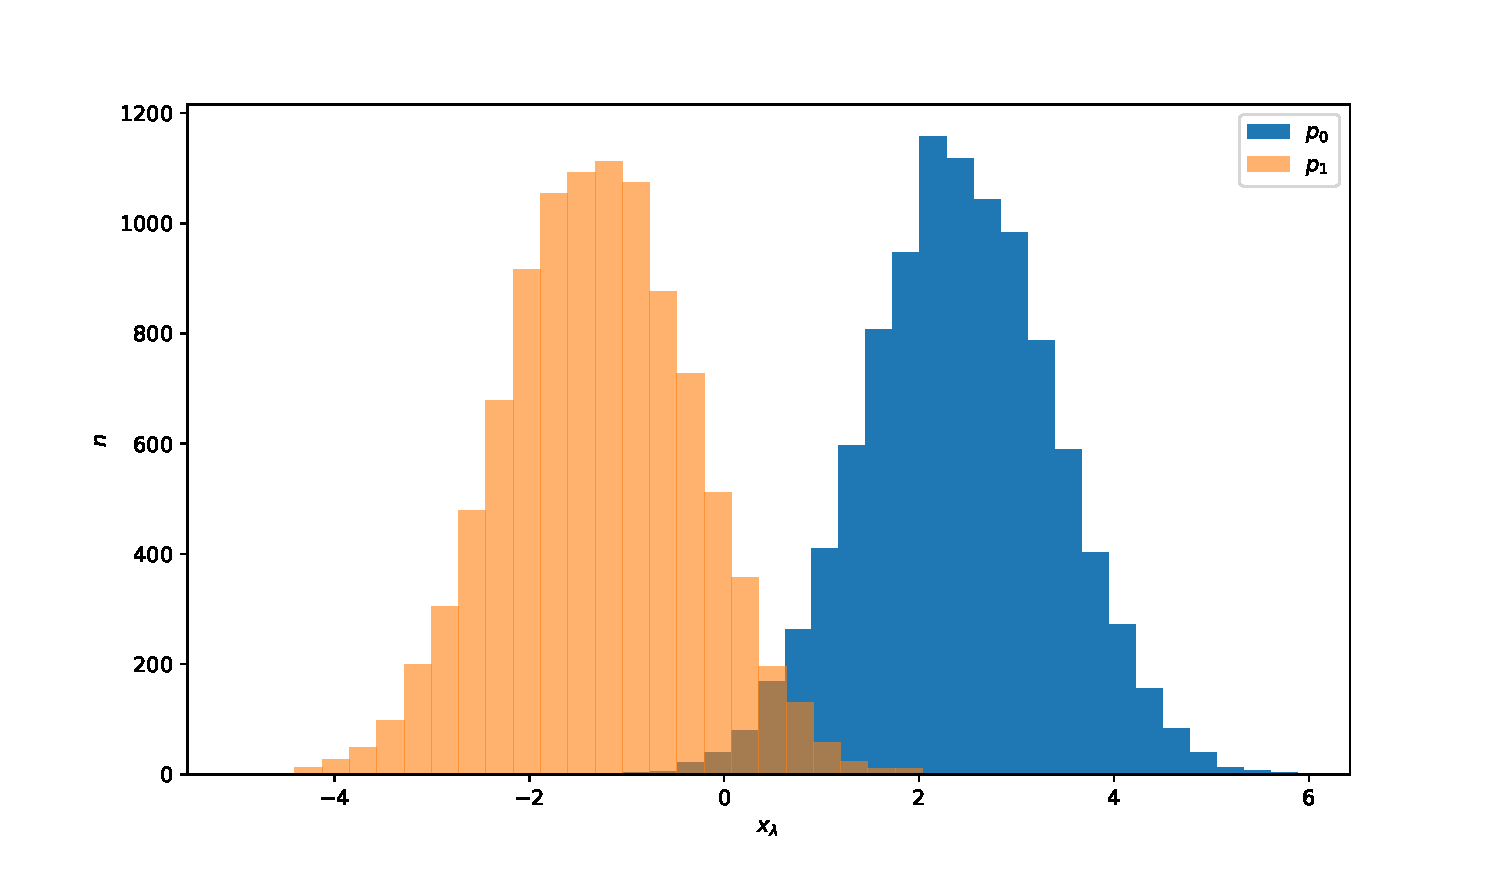
\includegraphics[width=\textwidth]{../A16/A16d_10000.pdf}
    \caption{Histogramm der Projektion für $P_{0, 10000}$.}
    \label{fig:A16d_10000}
\end{figure}
\begin{figure}
    \centering
    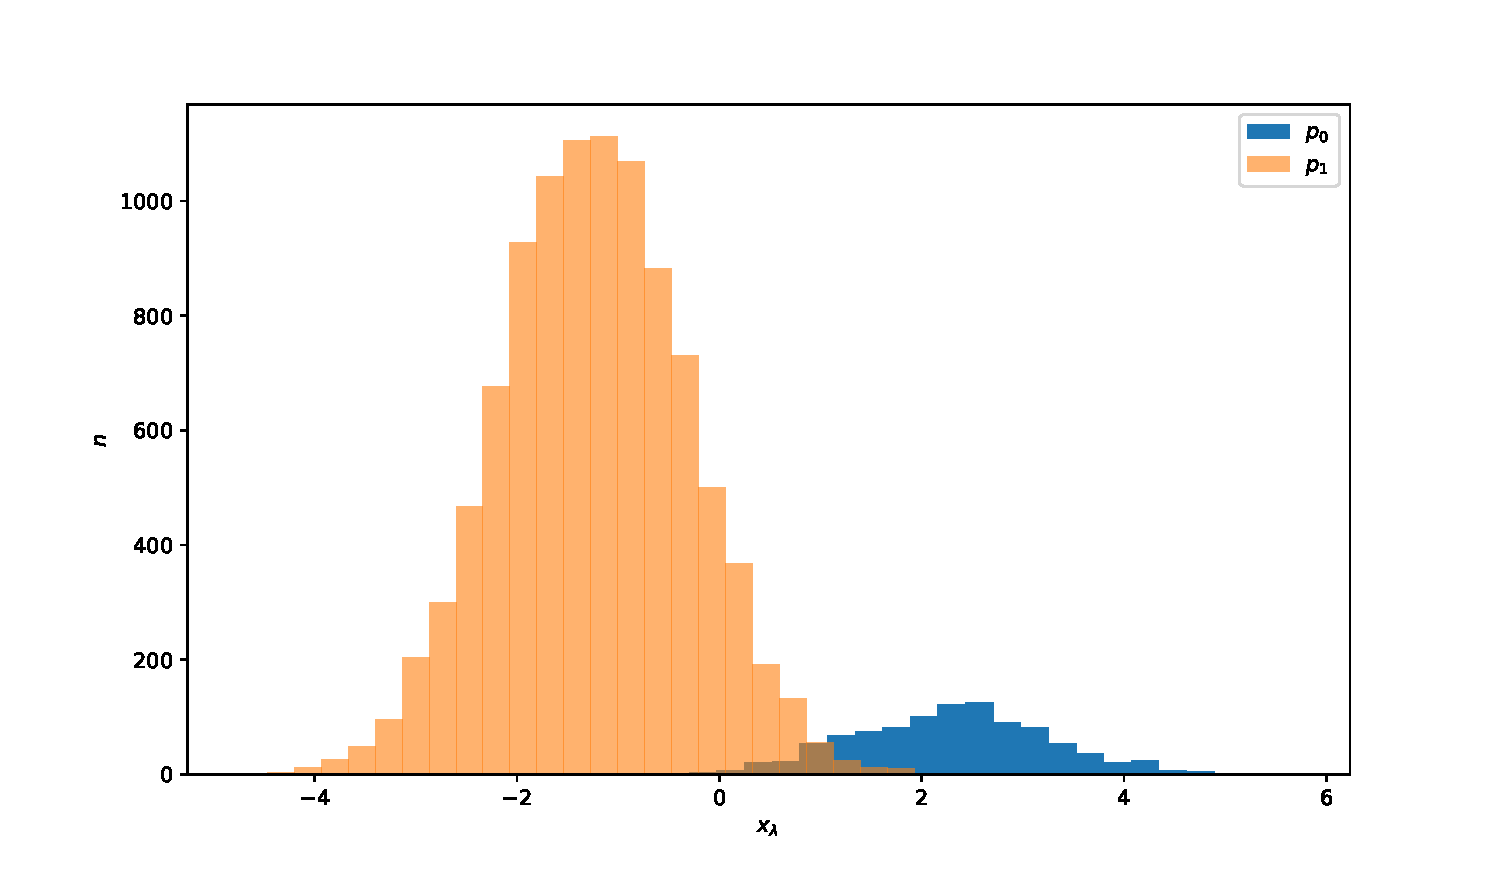
\includegraphics[width=\textwidth]{../A16/A16d_1000.pdf}
    \caption{Histogramm der Projektion für $P_{0, 1000}$.}
    \label{fig:A16d_1000}
\end{figure}
\FloatBarrier

\subsection*{e)}
\begin{figure}
    \centering
    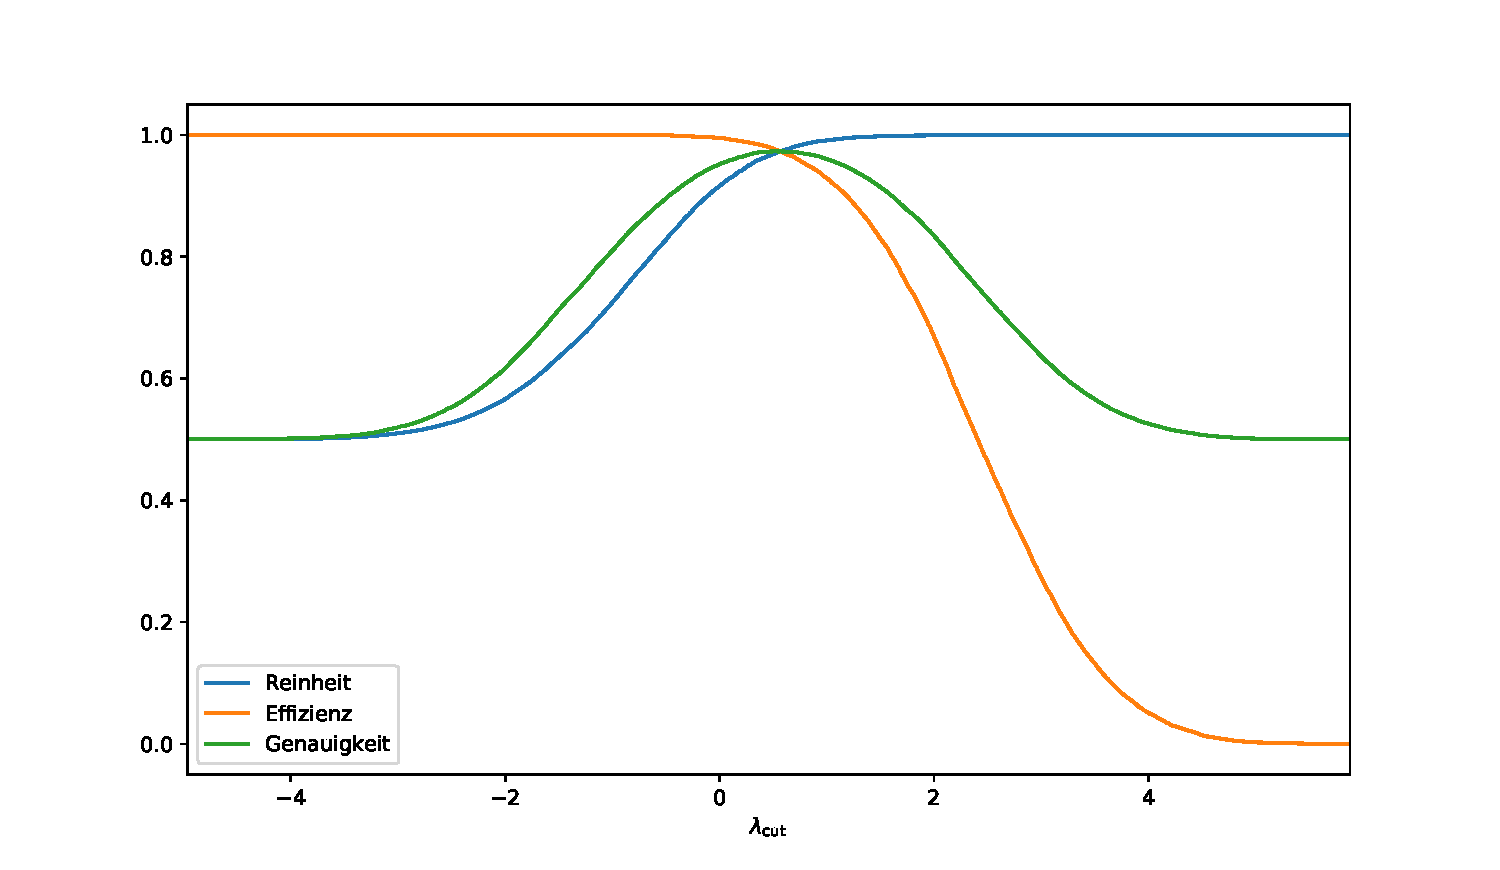
\includegraphics[width=\textwidth]{../A16/A16e_10000.pdf}
    \caption{Effizienz, Reinheit und Genauigkeit für $P_{0, 10000}$.}
    \label{fig:A16e_10000}
\end{figure}
\begin{figure}
    \centering
    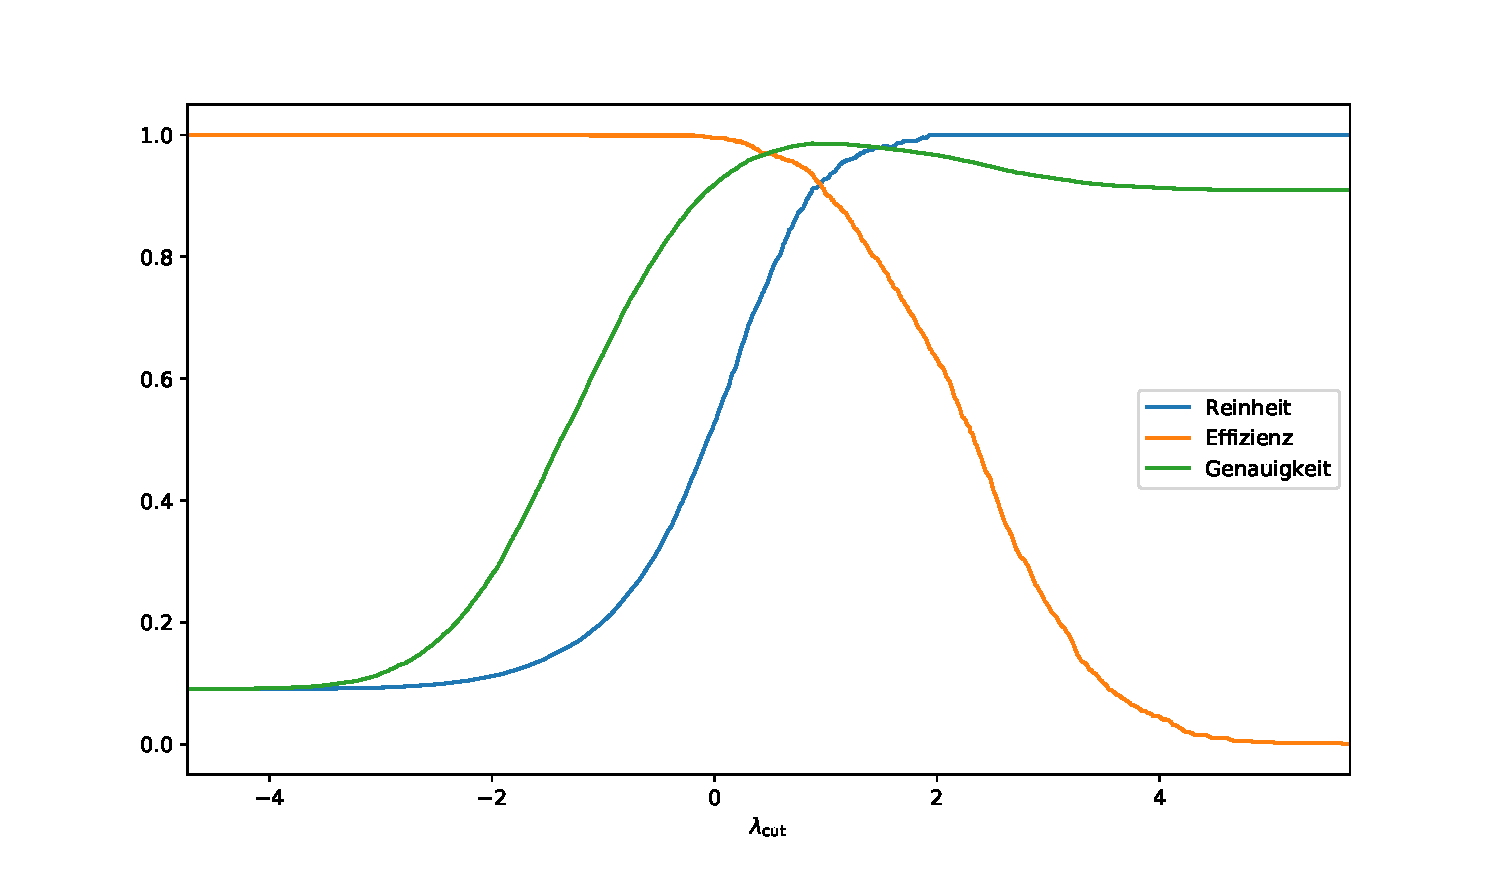
\includegraphics[width=\textwidth]{../A16/A16e_1000.pdf}
    \caption{Effizienz, Reinheit und Genauigkeit für $P_{0, 1000}$.}
    \label{fig:A16e_1000}
\end{figure}
\FloatBarrier

\subsection*{f)}
Das Signal-zu-Untergrundverhältnis $\frac{S}{B}$ wird maximal für $B \rightarrow 0$ also für $\lambda_\textup{cut} \rightarrow -\infty$.
\begin{figure}
    \centering
    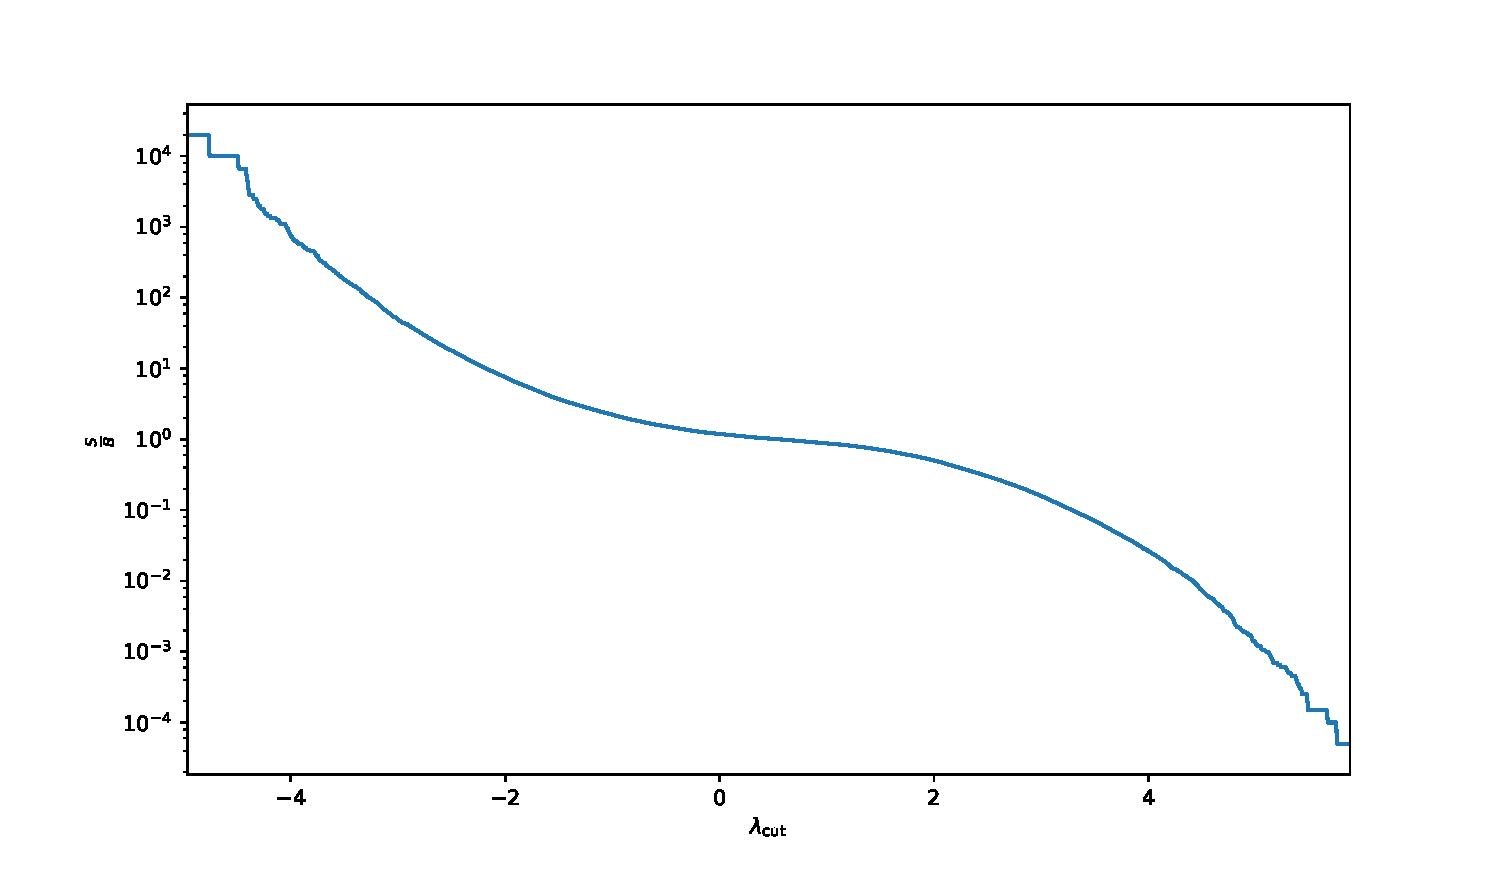
\includegraphics[width=\textwidth]{../A16/A16f_10000.pdf}
    \caption{Signal-zu-Untergrundverhältnis für $P_{0, 10000}$.}
    \label{fig:A16f_10000}
\end{figure}
\begin{figure}
    \centering
    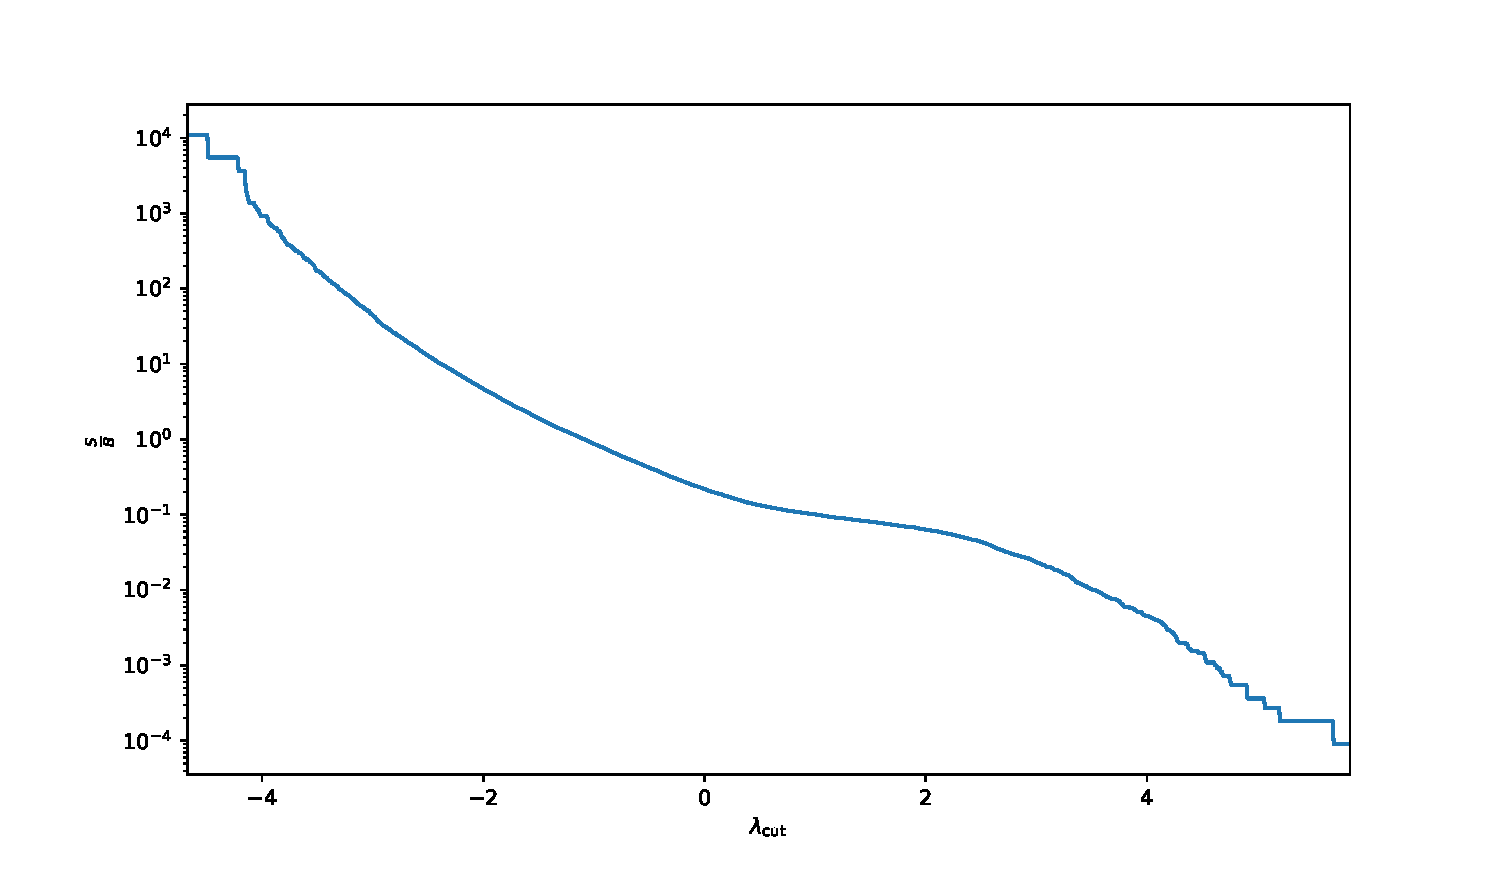
\includegraphics[width=\textwidth]{../A16/A16f_1000.pdf}
    \caption{Signal-zu-Untergrundverhältnis für $P_{0, 1000}$.}
    \label{fig:A16f_1000}
\end{figure}
\FloatBarrier

\subsection*{g)}
Die Signifikanz $\frac{S}{\sqrt{S + B}}$ wird maximal für $S + B \rightarrow 0$ also für $\lambda_\textup{cut} \rightarrow -\infty$.
\begin{figure}
    \centering
    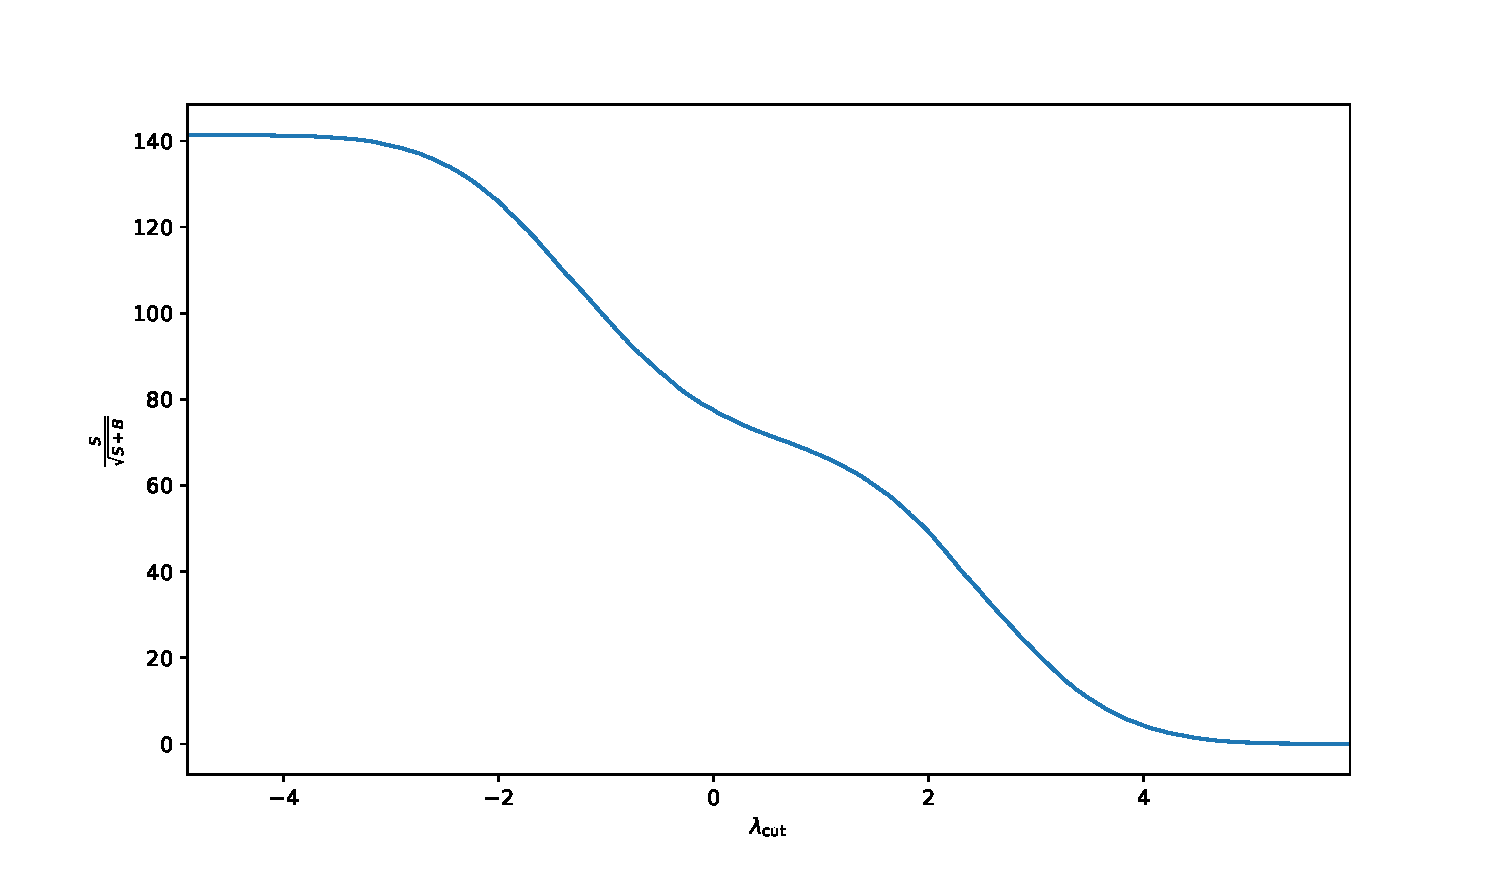
\includegraphics[width=\textwidth]{../A16/A16g_10000.pdf}
    \caption{Signifikanz für $P_{0, 10000}$.}
    \label{fig:A16g_10000}
\end{figure}
\begin{figure}
    \centering
    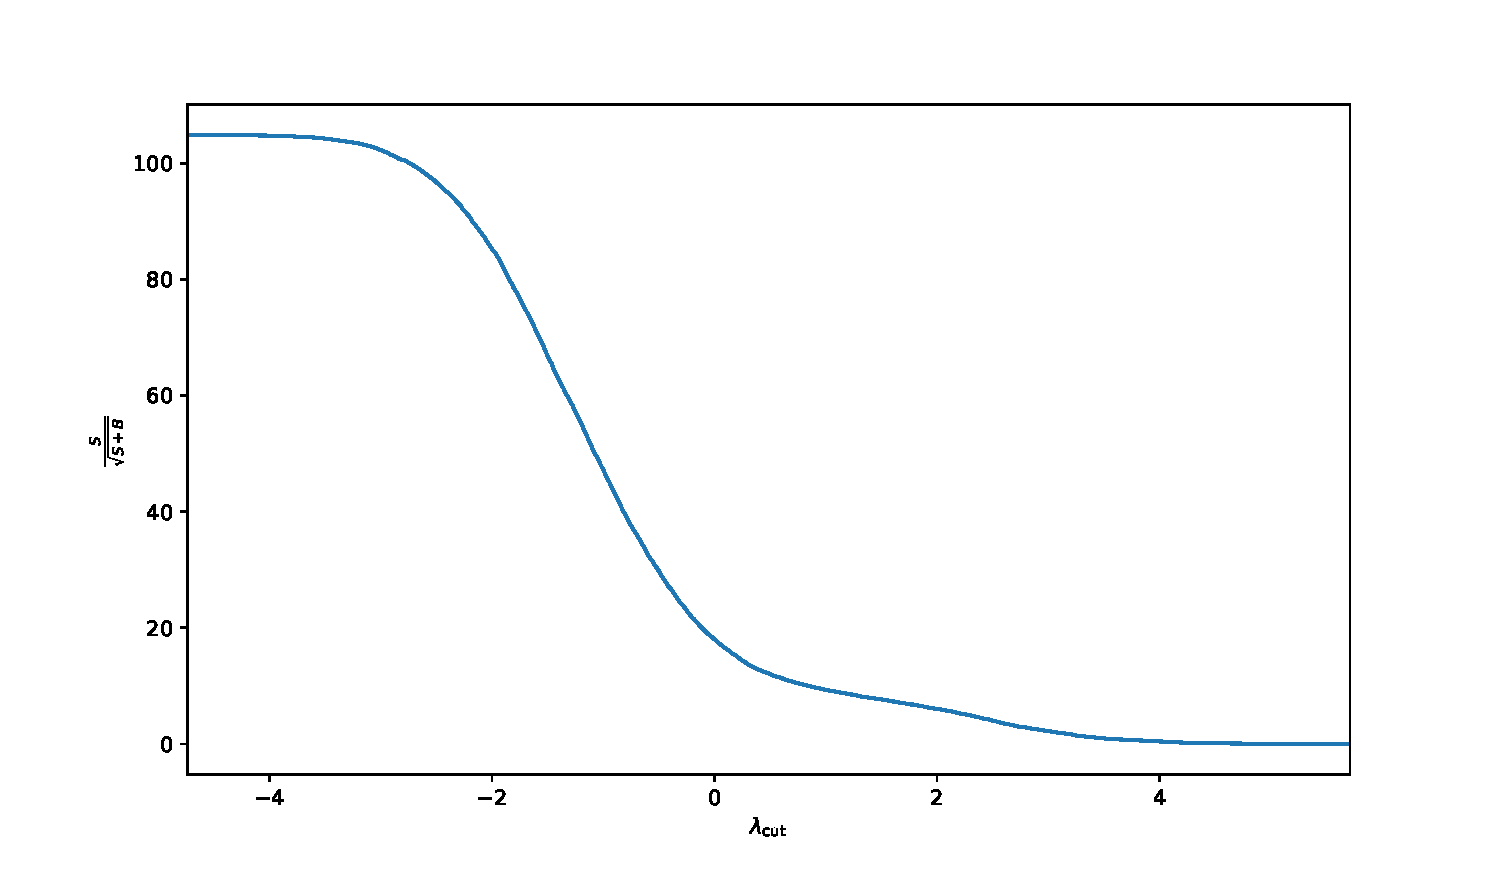
\includegraphics[width=\textwidth]{../A16/A16g_1000.pdf}
    \caption{Signifikanz für $P_{0, 1000}$.}
    \label{fig:A16g_1000}
\end{figure}
\FloatBarrier
\end{document}
